\subsubsection{Mô tả thuật toán phát sinh khóa}
\noindent\textbf{2.1.1\quad Yêu cầu}\\
- File cần crack: \texttt{WinCrackMe.exe}\\
- Công cụ: \texttt{OllyDbg}\\
\noindent\textbf{2.1.2\quad Hướng dẫn}\\
- Khởi động chương trình dưới dạng \texttt{teminal line}, lúc này chương trình sẽ hiển thị như sau:
\begin{center}
    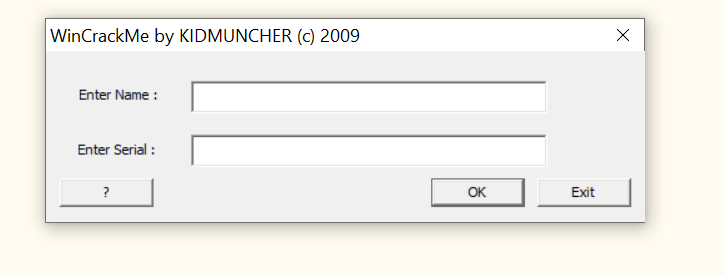
\includegraphics[width=\textwidth]{img/file-2/demo1.PNG}
\end{center}
- Chương trình hiển thị một  \texttt{hộp thoại dialog} chứa 2 thuộc tính cần được nhập vào: \texttt{Enter Name} và \texttt{Enter Serial}. Bên dưới cùng bên trái hiển thị \texttt{Button '?'} dùng để hiển thị thông báo \texttt{Instructions}, cung cấp thông tin về chương trình và tác giả. Bên dưới cùng bên phải hiển thị Button \texttt{OK} và \texttt{Exit}\\
\begin{center}
    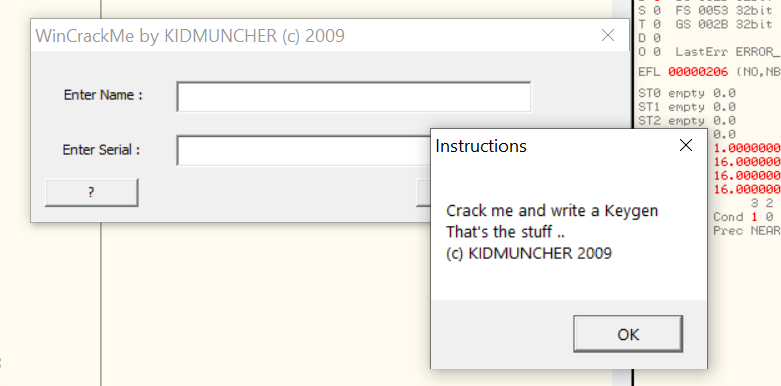
\includegraphics[width=\textwidth]{img/file-2/demo2.PNG}
\end{center}
- Xét các trường hợp có thể xảy ra dưới đây:\\
+ \textbf{TH1}: Để trống cả hai thuộc tính, kết quả trả về như sau:
\begin{center}
    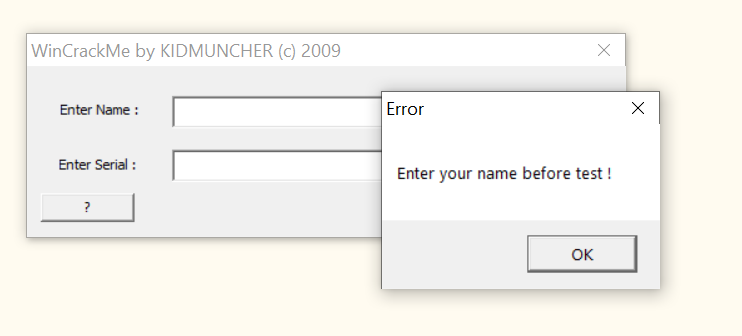
\includegraphics[width=\textwidth]{img/file-2/demo3.PNG}
\end{center}
+ \textbf{TH2}: Nhập vào thuộc tính \texttt{Name} một vài kí tự, số lượng chữ cái ít hơn 5, kết quả trả về như sau:
\begin{center}
    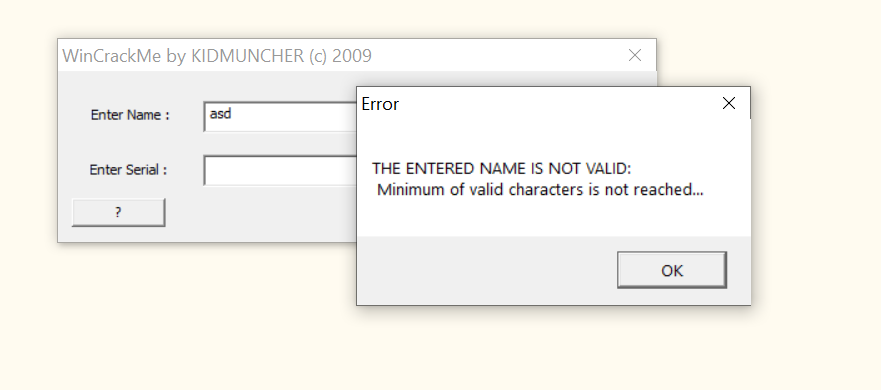
\includegraphics[width=\textwidth]{img/file-2/demo4.PNG}
\end{center}
+ \textbf{TH3}: Nhập vào thuộc tính \texttt{Name} các kí tự \texttt{a} hoặc \texttt{A}, số lượng chữ cái lớn hơn 5, kết quả trả về như sau:
\begin{center}
    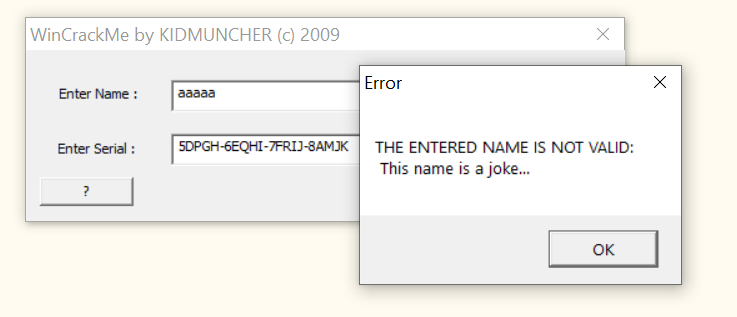
\includegraphics[width=\textwidth]{img/file-2/demo5.PNG}
\end{center}
+ \textbf{TH4}: Nhập vào thuộc tính \texttt{Name} các kí tự bất kì, số lượng chữ cái lớn hơn 5, kết quả trả về như sau:
\begin{center}
    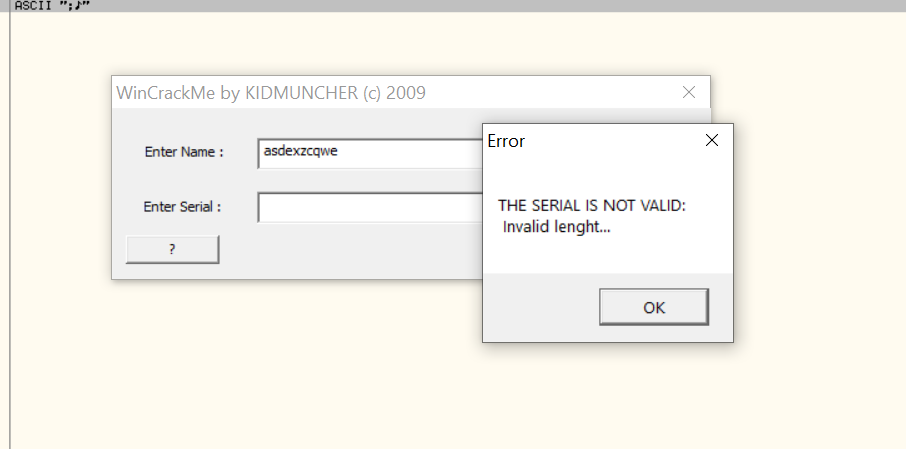
\includegraphics[width=\textwidth]{img/file-2/demo6.PNG}
\end{center}
+ \textbf{TH5}: Nhập vào thuộc tính \texttt{Serial} 1 vài kí tự bất kì, kết quả trả về như sau:
\begin{center}
    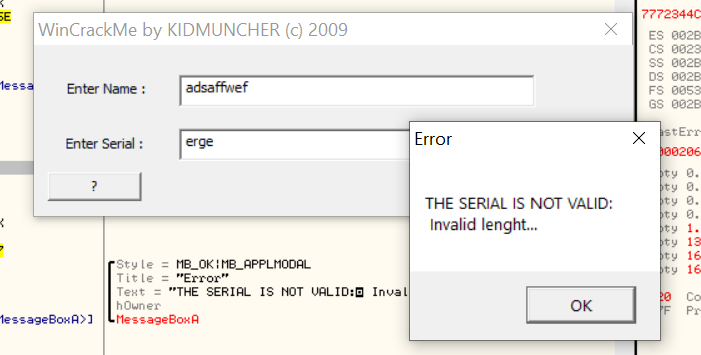
\includegraphics[width=\textwidth]{img/file-2/demo9.PNG}
\end{center}
+ \textbf{TH6}: Nhập vào thuộc tính \texttt{Serial} các kí tự bất kì, số lượng chữ cái đúng bằng 23, kết quả trả về như sau:
\begin{center}
    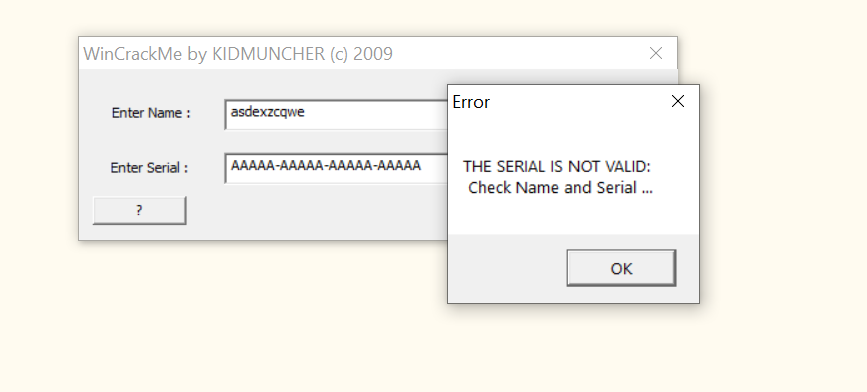
\includegraphics[width=\textwidth]{img/file-2/demo7.PNG}
\end{center}
+ \textbf{TH7}: Nhập vào thuộc tính \texttt{Serial} các kí tự tương ứng vỡi thuộc tính \texttt{Name} đã nhập vào, kết quả trả về như sau:
\begin{center}
    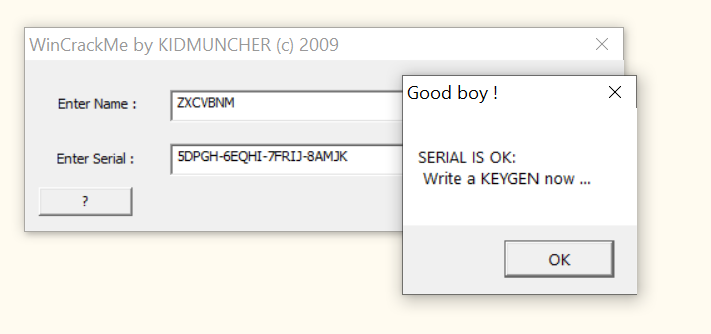
\includegraphics[width=\textwidth]{img/file-2/demo8.PNG}
\end{center}



\noindent\textbf{2.1.3\quad Chi tiết}\\
- Khởi động chương trình \texttt{OllyDbg} và mở file \texttt{WinCrackMe.exe}. Giao diện của chương trình sẽ như sau: 
\begin{center}
    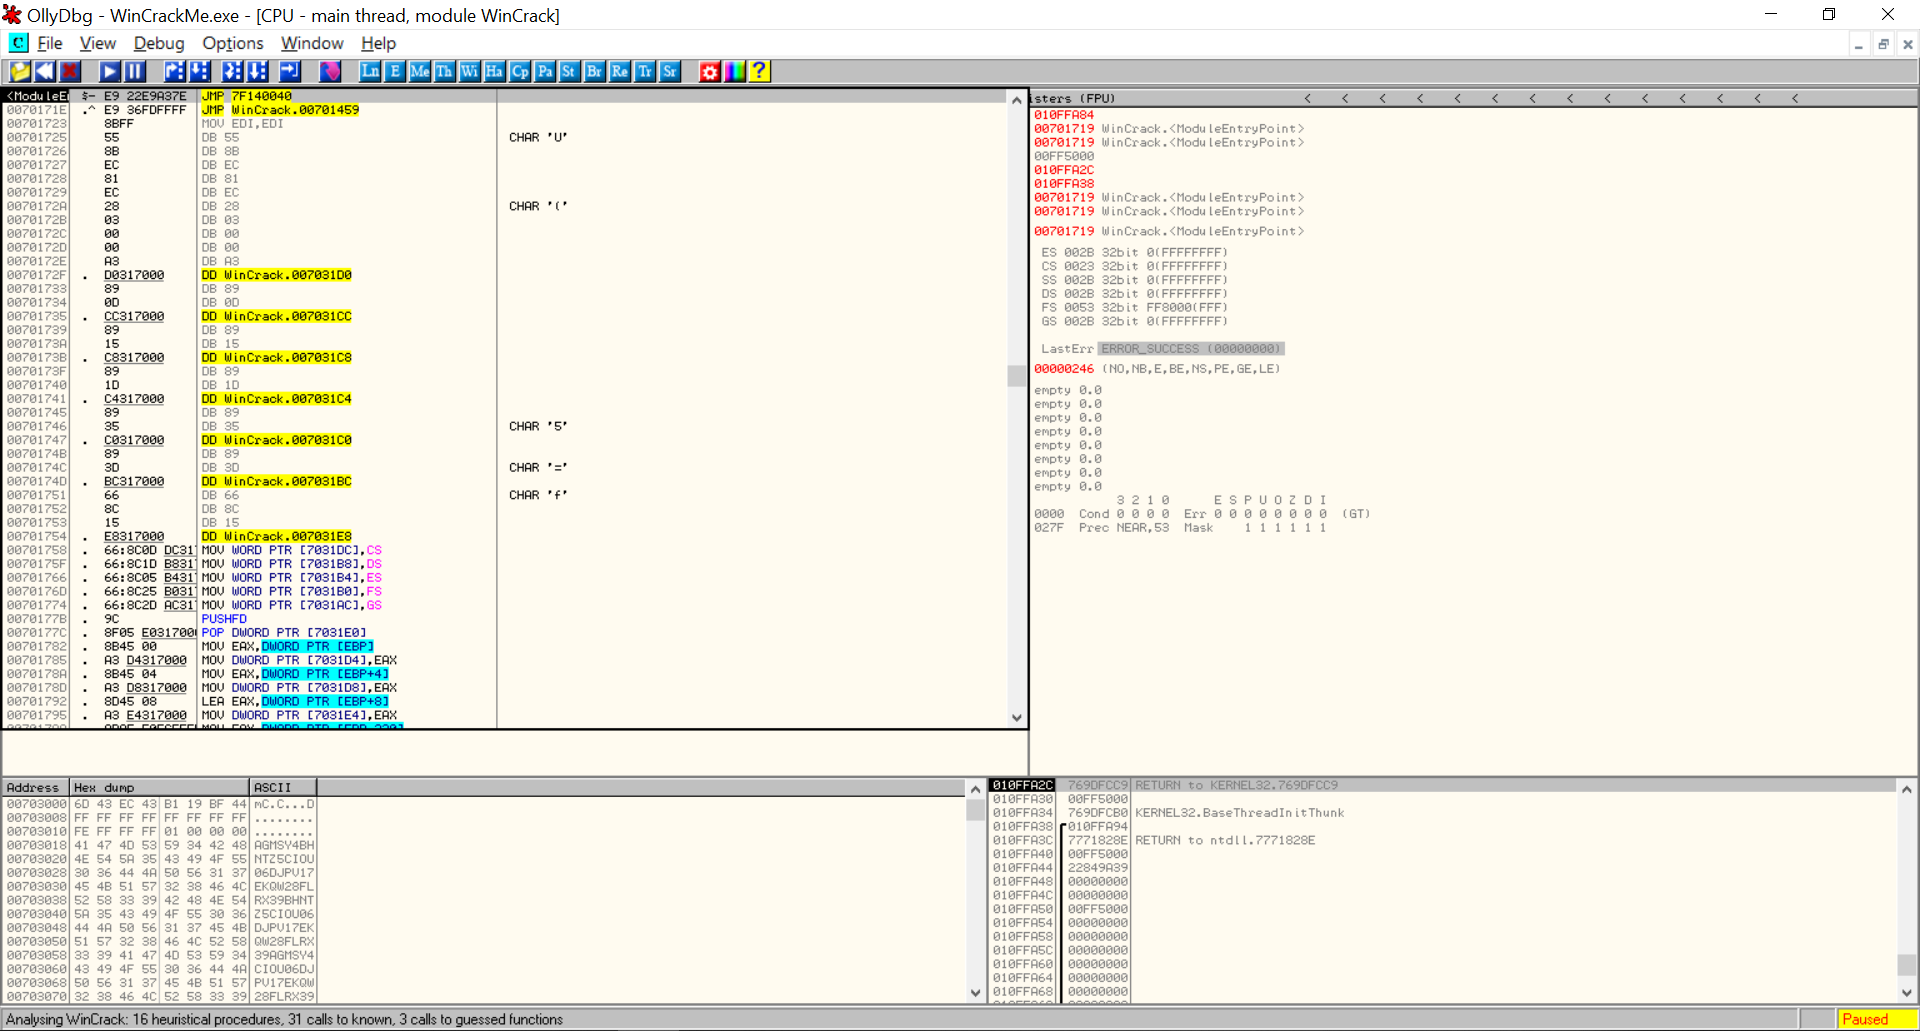
\includegraphics[width=\textwidth]{img/file-2/asm1.PNG}
\end{center}
- Click chuột phải, chọn \texttt{Search for>All references text strings}, lúc này chương trình sẽ hiển thị các dòng lệnh xuất thông báo ra màn hình.\\
\begin{center}
    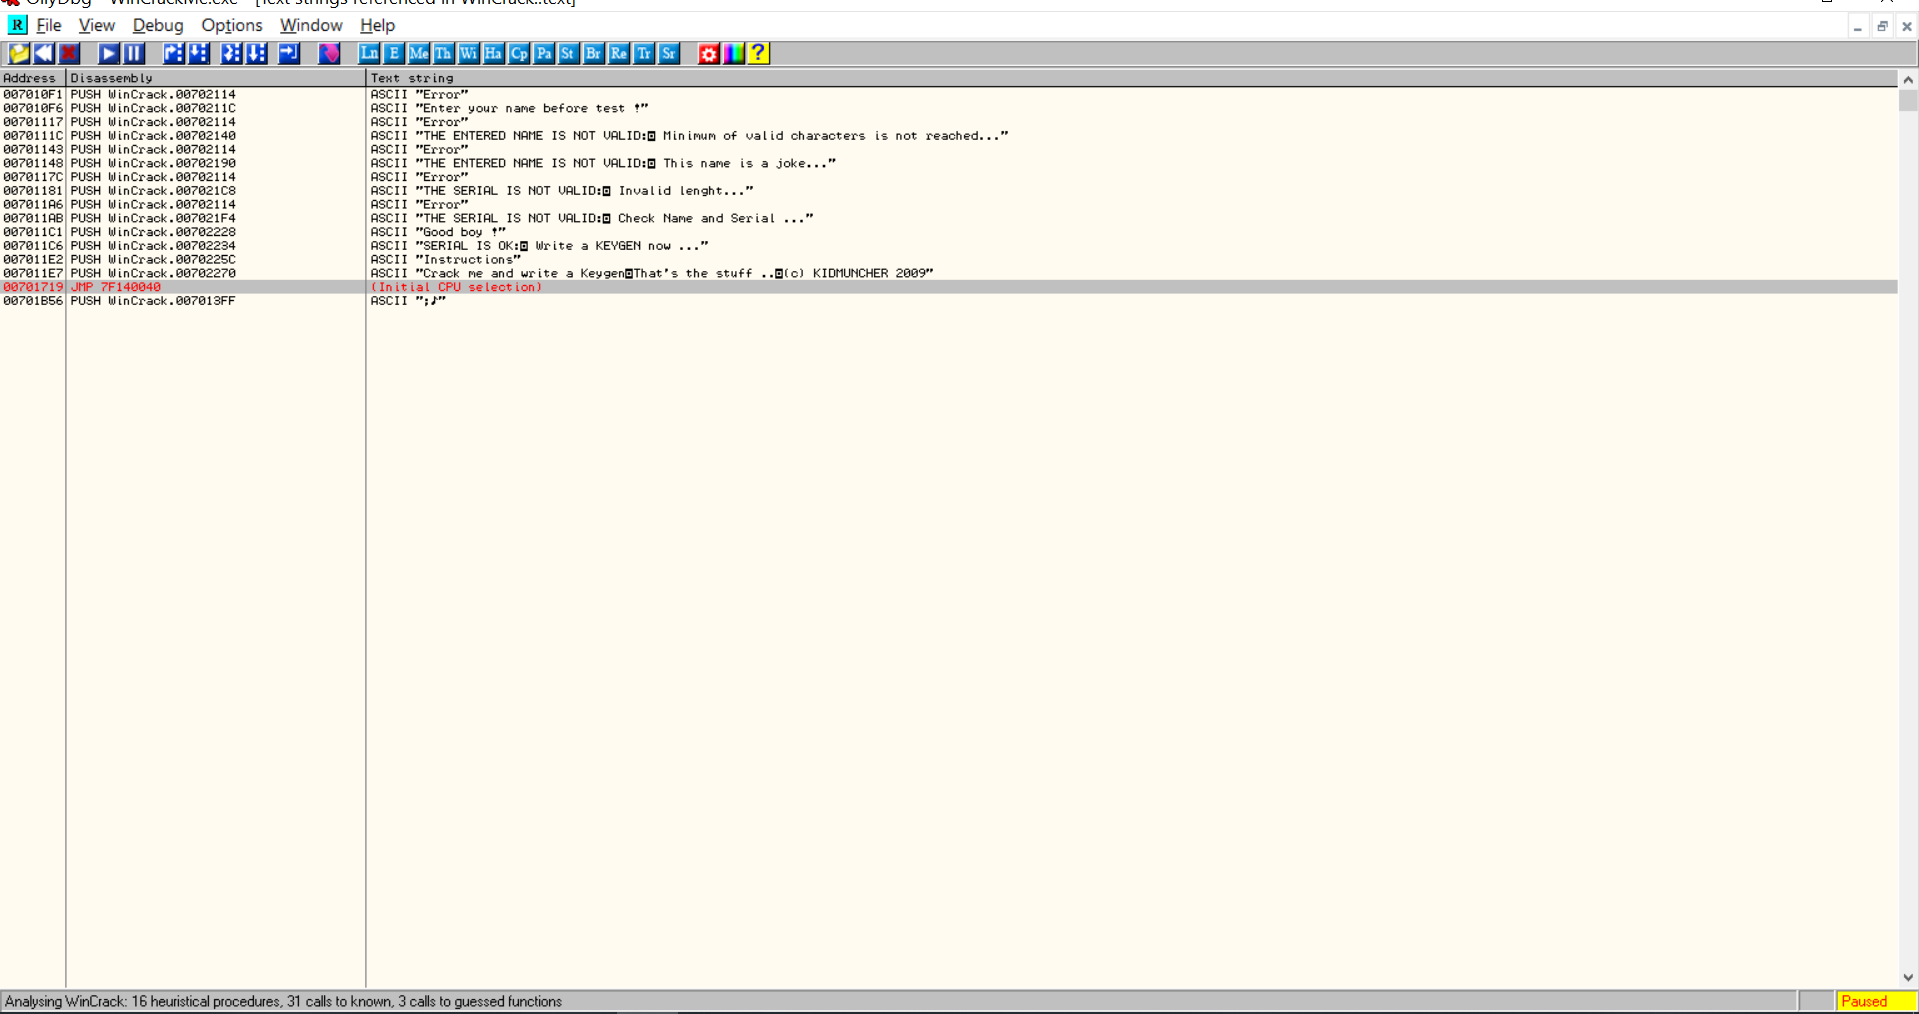
\includegraphics[width=\textwidth]{img/file-2/asm2.PNG}
\end{center}
- Double-click vào dòng đầu tiên trên màn hình. Lúc này đặt breakpoint tại vị trí đó để phân tích các bước thực thi của chương trình:\\
+ \textbf{Bước 1}: Nhập thông tin (nếu có) vào 2 thanh thuộc tính của chương trình và nhấn vào OK để tiếp tục. Chưởng trình sẽ đưa hàm \texttt{GetDlgItemTextA} vào thanh ghi \texttt{EDI} để gọi hàm lấy giá trị thuộc tính \texttt{name} và \texttt{Serial}\\
\begin{center}
    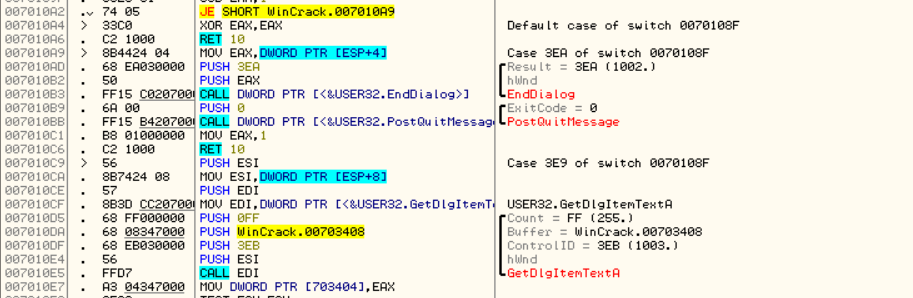
\includegraphics[width=\textwidth]{img/file-2/asm3.PNG}
\end{center}
+ \textbf{Bước 2}: Kiểm tra thuộc tính \texttt{name} có rỗng hay không? Chương trình sẽ kiểm tra bằng lệnh \texttt{TEST}. Lệnh \texttt{TEST} tương tự với lệnh \texttt{AND}, tuy nhiên khác với lệnh \texttt{AND} là sau khi thực hiện phép tính, giá trị sẽ không được lưu vào \texttt{OPERAND}1. Điều này cho phép chương trình so sánh 2 \texttt{OPERAND} mà không thay đổi giá trị của \texttt{OPERAND}. Do đó lệnh \texttt{TEST} thường dùng để so sánh các \texttt{OPERAND} và bật các bit flag tương ứng. Ở đây ta thấy lệnh \texttt{TEST EAX,EAX} sẽ thực hiện việc so sánh giá trị của thanh ghi EAX với chính nó, tuy nhiên mục đích của nó thực chất là kiểm tra xem giá trị của thanh ghi EAX có khác 0 hay không. Sau khi thực hiện lệnh \texttt{TEST} trên, bit \texttt{Z} sẽ bật lên nếu như thuộc tính \texttt{name} bằng 0, tức là rỗng. Lúc này chương trình sẽ báo "Error: Enter your \texttt{name} before test!"\\
\begin{center}
    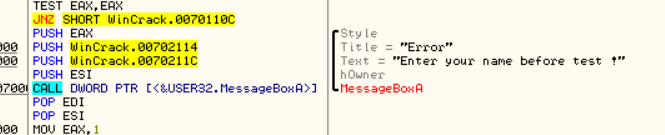
\includegraphics[width=\textwidth]{img/file-2/asm4.PNG}
\end{center}
+ \textbf{Bước 3}: Kiểm tra số từ có thỏa mãn điều kiện cho trước hay không? Chương trình sẽ kiểm tra số lượng phần tử tối thiểu trong thuộc tính \texttt{name}, sao cho số lượng chữ cái trong tên lớn hơn 4. Các chữ cái có thể là in hoa hoặc in thường, đồng thời trong tên có thể chứa các chữ số hoặc kí tự đặc biệt.\\
\begin{center}
    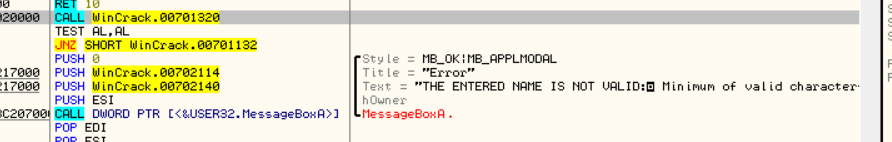
\includegraphics[width=\textwidth]{img/file-2/asm5.PNG}
\end{center}
+ \textbf{Bước 4}: Kiểm tra thuộc tính \texttt{name} có đủ điều kiện hay không?
Chương trình sẽ kiểm tra bằng cách băm thuộc tính \texttt{name} sử dụng hàm ở dưới. Chi tiết thuật toán sẽ ở phần \texttt{KEYGEN}:\\
\begin{center}
    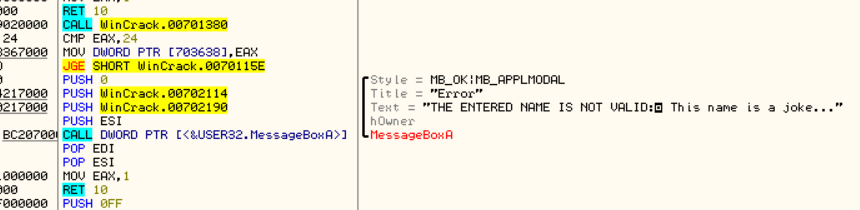
\includegraphics[width=\textwidth]{img/file-2/asm6.PNG}
\end{center}
+ \textbf{Bước 5}: Kiểm tra độ dài thuộc tính \texttt{Serial} có đủ hay không?
Chương trình sẽ kiểm tra số lượng kí tự trong thuộc tính \texttt{Serial} đúng bằng 23 kí tự không?\\
\begin{center}
    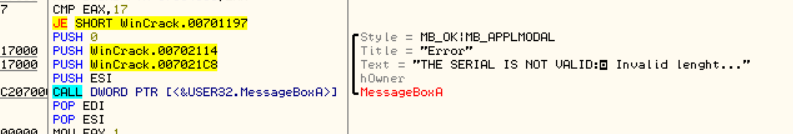
\includegraphics[width=\textwidth]{img/file-2/asm7.PNG}
\end{center}
+ \textbf{Bước 6}: Kiểm tra thuộc tính \texttt{Serial} có phù hợp không? Chương trình sủ dụng hàm băm để tính giá trị băm được.
Chương trình sẽ so sánh giá trị hash có được từ thuộc tính \texttt{Serial} với giá trị hash có được từ thuộc tính \texttt{name}. Chi tiết thuật toán sẽ ở phần KEYGEN\\
\begin{center}
    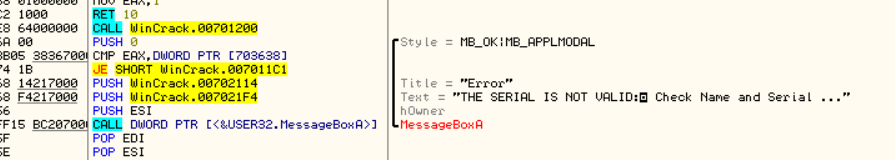
\includegraphics[width=\textwidth]{img/file-2/asm8.PNG}
\end{center}
+ \textbf{Bước 7}: Kết thúc. Chương trình hiển thị thông báo đã crack thành công\\
\begin{center}
    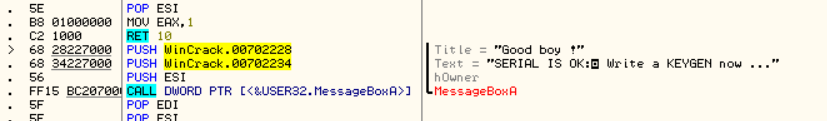
\includegraphics[width=\textwidth]{img/file-2/asm9.PNG}
\end{center}

\subsubsection{Chương trình phát sinh khóa}
- Chương trình phát sinh khóa dựa trên thuộc tính \texttt{name} đã cung cấp. Từ thuộc tính \texttt{name}, ta có được giá trị hash, và ta cần tìm khóa sao cho giá trị hash từ khóa bằng với giá trị hash từ \texttt{name}.\\
- Thuật toán tính giá trị hash của thuộc tính \texttt{name}:\\
+ Gán giá trị hash = 0, ta xét 5 chữ cái đầu tiên trong thuộc tính \texttt{name}: 
\[
    hash = hash*26 + index[ch[i]]
\]
+ Với từng kí tự, ta lấy giá trị của chúng trong bảng chữ cái không phân biệt hoa thường:
\[
    index[ch[i]] = lower(ch[i]) - 'a'
\]
\begin{center}
    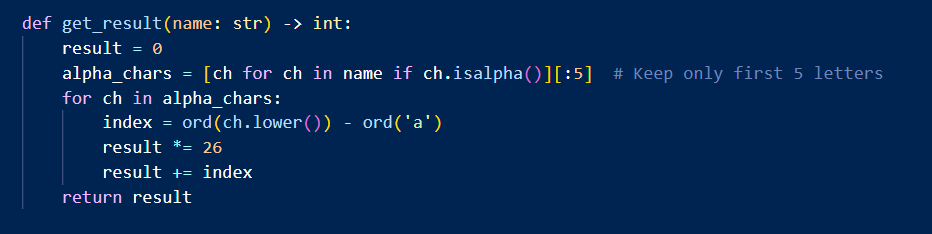
\includegraphics[width=\textwidth]{img/file-2/code1.PNG}
\end{center}

- Thuật toán tính giá trị hash của thuộc tính \texttt{Serial}:\\
+ Từ một dãy 23 ký tự, ta tách ra thành 4 khoảng có độ dài là 5, cách nhau bởi 1 kí tự đặc biệt. Các ký tự trong mỗi khoảng đều là các chữ cái in hoa hoặc các chữ số. Ex: \texttt{Serial} có thể là "AJVWI-2KLE0-6N563-MXNWE". \\
+ Trong chương trình có một bảng băm chứa 36 ký tự tương ứng với 26 ký tự chữ cái in hoa và 10 ký tự chữ số được lưu trữ một cách ngẫu nhiên, và giá trị của từng ký tự trong bảng băm chính là vị trí của nó trong đó, bắt đầu từ vị trí 0.\\
+ Trong chương trình có 4 bảng băm, tương ứng với 4 khoảng của \texttt{Serial}, với mỗi bảng băm đều bị dịch chuyển một đoạn so với bảng băm gốc, do đó ta cần băm các khoảng của \texttt{Serial} tương ứng với từng khoảng dịch chuyển của bảng băm tương ứng\\
\begin{center}
    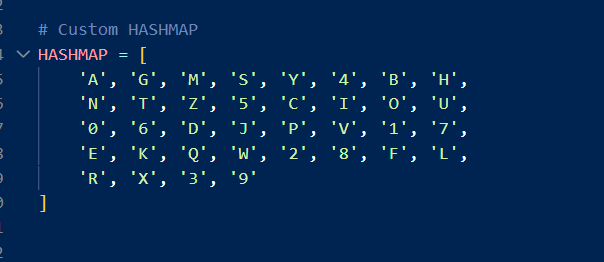
\includegraphics[width=\textwidth]{img/file-2/code2.PNG}
\end{center}
+ Giá trị của từng khoảng được tính như sau:
Đặt hash = 0, duyệt các phần tử từ phải qua.\\
\[
    index = gethash(ch[i])
\]
\[
    temp = hash
\]
\[
    tenp = temp * 9
\]
\[
    index = index + temp * 4
\]
\[
    hash = index
\]

\begin{center}
    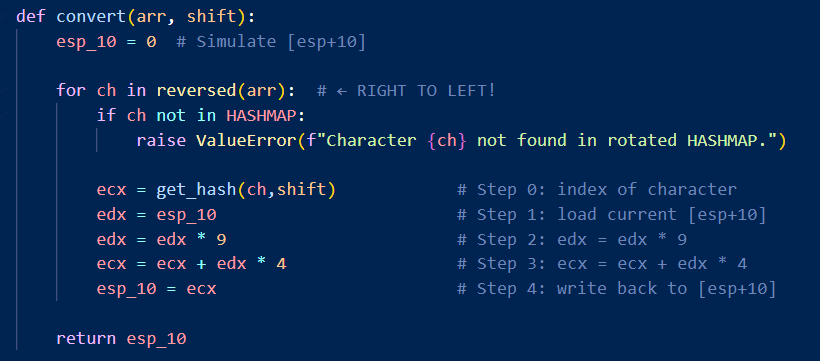
\includegraphics[width=\textwidth]{img/file-2/code3.PNG}
\end{center}

+ Ta so sánh giá trị hash của các khoảng với nhau. Điều kiện để thỏa yêu cầu là các giá trị hash của mỗi khoảng phải bằng nhau. Cuối cùng là so sánh với giá trị hash của thuộc tính \texttt{Name} rồi trả về kết quả

+ Chương trình \texttt{GENKEY} sử dụng \texttt{Greedy Algorithm} (thuật toán tham lam) để tìm giá trị lớn nhất của thuộc tính \texttt{Serial} dựa trên giá trị hash của thuộc tính \texttt{Name}. Lưu ý rằng có thể có nhiều giá trị thỏa mãn các điều kiện đã đặt ra ở trên, tuy nhiên chương trình GENKY chỉ trả về 1 giá trị \texttt{Serial} tương ứng với mỗi giá trị \texttt{Name} mà người dùng nhập vào. Kết quả sẽ được lưu vào trong file key.txt

\subsubsection{Kết luận}
- Chương trình trên sử dụng kỹ thuật băm (hashing) để mã hóa dữ liệu mà người dùng nhập vào. Khi đó giá trị \texttt{Name} và \texttt{Serial} được băm thành các giá trị hash dùng cho việc bảo mật dữ liệu, kiểm tra tính hợp lệ của dữ liệu đầu vào, hoặc để so sánh với các giá trị đã lưu trữ từ trước.